%\documentclass[a4paper,11pt]{article}
\documentclass{article}
%%%%%%%%%%%%%%%%%%%%%%%%%%%%%%%%%%%%%%%%%%%%%%%%%%%%%%%%%%%%%%%%%%%%%%%%%%%%%%%%%%%%%%%%%%%%%%%%%%%%%%%%%%%%%%%%%%%%%%%%%%%%
\usepackage{graphics,graphicx}
\usepackage{amsmath,amssymb,graphics,graphicx}
\usepackage[ansinew]{inputenc}
\usepackage[usenames,dvipsnames]{color}

\graphicspath{{Images/}}
\usepackage{natbib}

\bibpunct{(}{)}{;}{a}{,}{,}

\textheight 24cm \textwidth 17cm \topmargin-2cm
%% \evensidemargin   -0.25cm
\oddsidemargin-0.2cm
%\pagestyle{empty}
\renewcommand{\baselinestretch}{1}

\begin{document}

\title{Pr\'actica 1: FIFA Players Classification}

\author{{Daniel Carmona Pedrajas}}

\date{}
\maketitle

%\title{}

%\address{}

	\section{Arquitectura 1: One Layer Neural Network}
		Comenzamos los experimentos usando la siguiente arquitectura:
		\begin{enumerate}
			\item Capa densa con 512 neuronas.
		\end{enumerate}
		\subsection{Experimento 1}
		\label{s-a1-e1}
			Usamos la siguiente configuraci\'on:
			\begin{table}[h]
				\begin{center}
					\begin{tabular}{| c | c | c | c | c | c | c |}
						\textbf{Epochs} & \textbf{Learning rate} & \textbf{Batch size} & \textbf{Activation} & \textbf{Loss} & \textbf{Optimizer} & \textbf{Regularization} \\ \hline
						100 & 0.1 & 512 & ReLU & Categorical Crossentropy & SGD & None
					\end{tabular}
					\caption{Hiperpar\'ametros para el Experimento 1 de la Arquitectura 1}
					\label{tab:hip-a1-e1}
				\end{center}
			\end{table}
		
			Y entrenamos 5 veces para obtener los siguientes resultados:
			\begin{table}[h]
				\begin{center}
					\begin{tabular}{ c | c | c | c | c | c |}
						\ & \textbf{Train accuracy (\%)} & \textbf{Validation accuracy (\%)} & \textbf{Bias (\%)} & \textbf{Variance (\%)} & \textbf{Training time (s)} \\ \hline
						\textbf{Mean} & 79.38 & 77.94 & 15.61 & 1.44 & 14\\ \hline
						\textbf{Std} & 0.05 & 0.14 & 0.05 & 0.19 & 0 \\ \hline
					\end{tabular}
					\caption{Resultados del Experimento 1 de la Arquitectura 1}
					\label{tab:res-a1-e1}
				\end{center}
			\end{table}
		
			Tener un \textit{bias} alto y una \textit{variance} baja significa que hay margen de mejora antes de llegar al overfitting y hay varias posibilidades para conseguir una mejor \textit{accuracy}: a\~nadir m\'as capas o neuronas, entrenar con m\'as epochs, ...
		
		\subsection{Experimento 2}
		\label{s-a1-e2}
			Tras el experimento anterior, decidimos entrenar el modelo durante m\'as epochs para reducir el \textit{bias} usando la misma configuraci\'on.\\
			\begin{table}[h]
			\begin{center}
				\begin{tabular}{| c | c | c | c | c | c | c |}
					\textbf{Epochs} & \textbf{Learning rate} & \textbf{Batch size} & \textbf{Activation} & \textbf{Loss} & \textbf{Optimizer} & \textbf{Regularization} \\ \hline
					1000 & 0.1 & 512 & ReLU & Categorical Crossentropy & SGD & None
				\end{tabular}
				\caption{Hiperpar\'ametros para el Experimento 2 de la Arquitectura 1}
				\label{tab:hip-a1-e2}
			\end{center}
		\end{table}
			
			Tras 5 entrenamientos obtenemos los siguientes resultados:
			\begin{table}[!h]
			\begin{center}
				\begin{tabular}{ c | c | c | c | c | c |}
					\ & \textbf{Train accuracy (\%)} & \textbf{Validation accuracy (\%)} & \textbf{Bias (\%)} & \textbf{Variance (\%)} & \textbf{Training time (s)} \\ \hline
					\textbf{Mean} & 84.02 & 81.5 & 10.97 & 2.47 & 199\\ \hline
					\textbf{Std} & 0.03 & 0.17 & 0.03 & 0.18 & 8.8 \\ \hline
				\end{tabular}
				\caption{Resultados del Experimento 2 de la Arquitectura 1}
				\label{tab:res-a1-e2}
			\end{center}
		\end{table}
			Con respecto al experimento anterior hemos aumentado el \textit{accuracy} tanto en el entrenamiento como en validaci\'on, reduciendo as\'i el \textit{bias} del modelo en un 5\% aunque ha aumentado ligeramente el \textit{variance}. Como es l\'ogico el tiempo de entrenamiento ha crecido, aunque no de forma lineal.\\
			\begin{figure}[!h]
				\begin{center}
					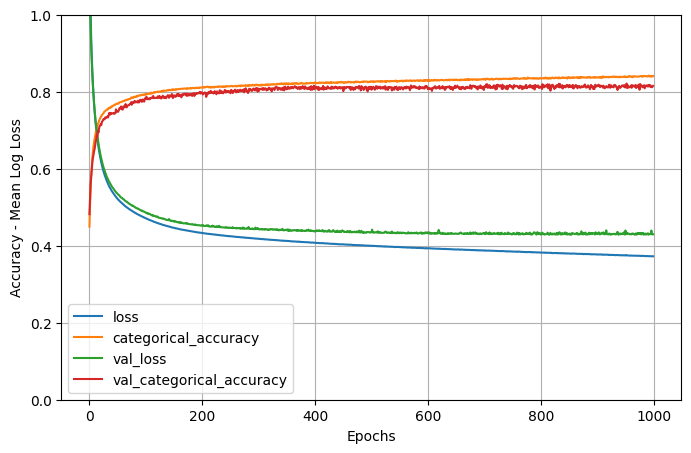
\includegraphics[scale=0.5]{exp1-2.png}		
					\caption{Entrenamiento durante el Experimento 2 de la Arquitectura 1}	
					\label{tr-a1-e2}
				\end{center}
			\end{figure}
			Como se ve en la figura \ref{tr-a1-e2}, a partir del epoch 400 no hay una mejora en \textit{accuracy} para el conjunto de validaci\'on aunque s\'i para el conjunto de entrenamiento lo que nos indica que un n\'umero de epochs tan elevado como el que hemos usado en este experimento con esta arquitectura conduce a un overfitting del modelo, aunque por el momento no es excesivo como nos indica la \textit{variance}.
			
		\subsection{Experimento 3}
		\label{s-a1-e3}
			Para este experimento decidimos reducir las epochs ya que como hemos visto en el experimento anterior, no hay una mejora significativa en validaci\'on con m\'as epochs.\\
			Adem\'as de esto, cambiaremos la funci\'on de activaci\'on a \textit{tanh} ya que hasta el momento hemos usado \textit{ReLU} pero no hay motivo de usarla en esta arquitectura porque resuelve el problema del \textit{vanishing gradient} que se da en arquitecturas profundas.\\
			La configuraci\'on que usamos para el experimento 3 es:
			

			
\end{document}
